\documentclass[10pt,a4paper,twocolumn]{article}
\usepackage[utf8]{inputenc}

\usepackage{siunitx}

\usepackage{graphicx}

\usepackage{tikz}
\usetikzlibrary{arrows,shapes,backgrounds, positioning, intersections, decorations.markings, decorations.shapes, mindmap, shapes.geometric, matrix, patterns}

\tikzset{lab/.style={above right, inner sep=0, font=\sffamily\Large\bfseries}}

\usepackage{pgfplots}

\pgfplotsset{every axis/.append style={xlabel near ticks,ylabel near ticks,mark size={0.2em}}}

\definecolor{Main}{rgb}{1, 0.57, 0}
\definecolor{Accent1}{rgb}{1,0.28,0}
\definecolor{Accent2}{rgb}{1,0.74,0}


\author{Mathieu Leocmach}
\begin{document}

\begin{figure}
	\begin{tikzpicture}
	\begin{axis}[%
		name=pH,
		xmin=0,xmax=8,
		ymin=0, ymax=7,
		xlabel={time (h)}, ylabel={\textcolor{Accent1}{pH}},
		extra tick style={grid=major},%
		extra y ticks={4.6}, extra y tick labels={},%
		extra x ticks={0.55, 0.64, 0.72, 0.80, 1, 1.27, 2.5}, extra x tick labels={},%
		axis y line*=left,
		width=0.925\columnwidth,
		height=0.5\columnwidth,
		]
	\addplot+[no marks,Accent1] table[x expr={\thisrowno{0}/3600.+0.05}]{Y189_28800s.pH};
	\node[base left=0] at (axis cs:8,4.6) {isoelectric};
	\end{axis}
	\begin{axis}[%
		xmin=0,xmax=8,
		ymin=0,
		ylabel=\textcolor{Accent2}{$G^\prime$ (\si{\pascal})},
		axis y line*=right,
		axis x line=none,
		width=0.925\columnwidth,
		height=0.5\columnwidth,
		]
	\addplot+[no marks,Accent2] table[x expr={\thisrowno{0}/3600.+0.05}]{Y235_28800s.prise};
	\end{axis}
	\node[lab, yshift=0.5em] at (pH.outer south west) {a};
	\begin{scope}[shift=(pH.outer south west), yshift=-2em]
		\fill[pattern=north east lines,pattern color=Accent2] (0,0) rectangle (\columnwidth,1.5em) node[midway,fill=white,inner sep=1pt] {glass};
		\fill[pattern=north east lines,pattern color=Accent2] (0,-2.5em) rectangle (\columnwidth,-4em) node[midway,fill=white,inner sep=1pt] {glass};
		\draw[line width=2pt,Accent1] (0.05\columnwidth,-2.5em) -- (0.95\columnwidth,-2.5em) (0.05\columnwidth,-1pt) -- (0.95\columnwidth,-1pt) node[pos=0, below right, inner sep=1pt, text width=0.4\columnwidth] {acrylamide brush ($10\sim \SI{100}{\nano\metre}$)};
		\fill[gray] (0,0) rectangle (0.05\columnwidth,-2.5em) (\columnwidth,0) rectangle (0.95\columnwidth,-2.5em) node[pos=1, above left] {spacer};
		\draw[<->] (0.75\columnwidth,-2pt) -- (0.75\columnwidth,-2.5em) node[midway,left] {$e\sim \SI{100}{\micro\metre}$};
		\draw[<->] (0.05\columnwidth,-4.25em) -- (0.95\columnwidth,-4.25em) node[midway,below] (L) {$L\sim\SI{2}{\centi\metre}$};
		\node[lab] at (0,0 |- L.base) {b};
	\end{scope}
	\begin{scope}[inner sep=0, shift=(pH.outer south west), yshift=-10.5em]
		\node[anchor=west] (a) {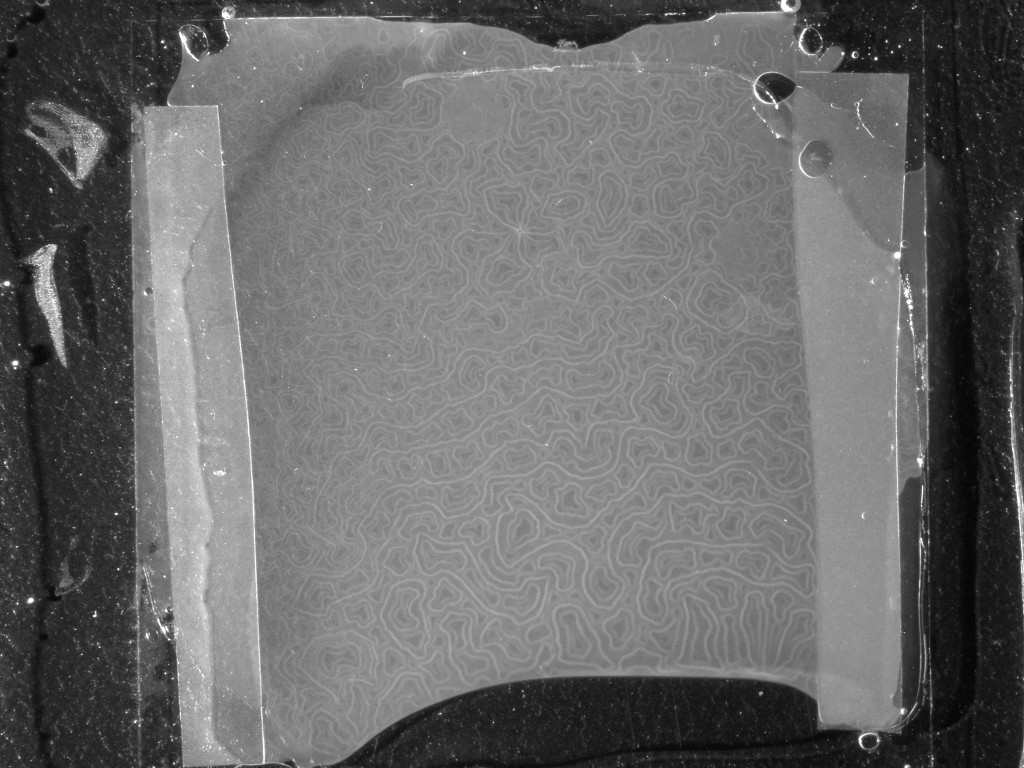
\includegraphics[width=0.3\columnwidth]{cas3p2_fluo0p8_GDL4_50um_coating_2_zoom2}};
		\node at (0.5\columnwidth,0) (b) {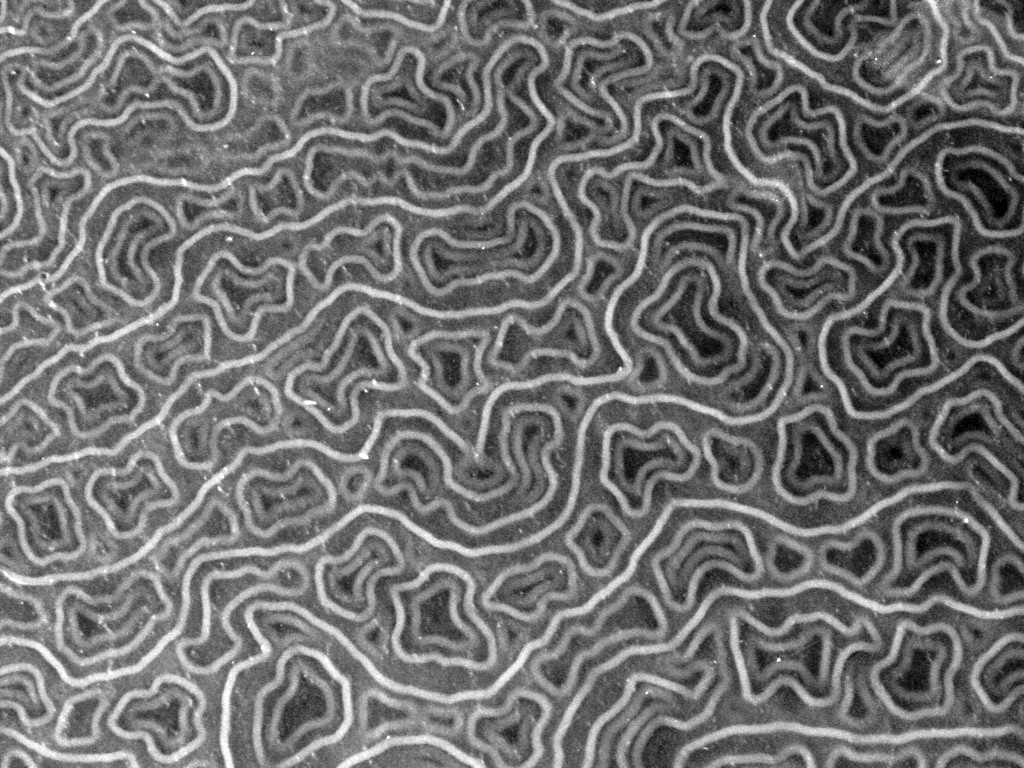
\includegraphics[width=0.3\columnwidth]{cas3p2_fluo0p8_GDL4_50um_coating_2_zoom6}};
		\node[anchor=east] at (\columnwidth,0) (c) {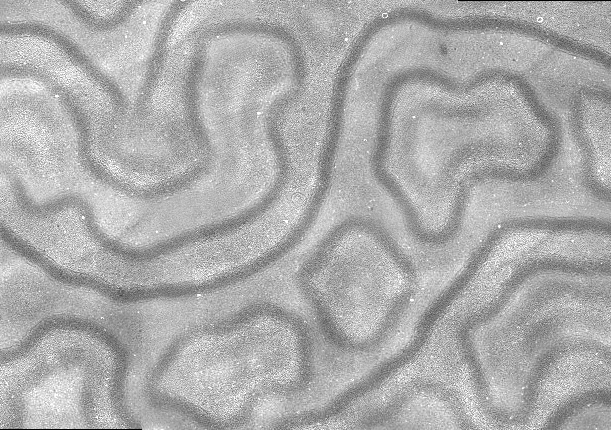
\includegraphics[width=0.3\columnwidth]{cas3p2_fluo0p8_GDL4_50um_coating_2_transmission}};
		\draw[Accent2] (a.north west) ++(0.126\columnwidth, -0.086\columnwidth) rectangle +(0.1\columnwidth,-0.075\columnwidth) -- (b.south west) (a.north west) ++(0.226\columnwidth, -0.086\columnwidth) -- (b.north west);
		\draw[Main] (b.north west) ++(0.117\columnwidth,-0.117\columnwidth) rectangle +(0.093\columnwidth,-0.068\columnwidth) -- (c.south west) (b.north west) ++(0.211\columnwidth,-0.117\columnwidth) --(c.north west);
		\draw[Accent1] (c.north west) ++(0.094\columnwidth,0) rectangle +(0.117\columnwidth,-0.117\columnwidth);
		\draw[ultra thick] (a.south east) ++(0,-0.25em) -- ++(-0.106\columnwidth,0) node[pos=0.5, below=0.25em, font=\small] (M) {\SI{1}{\centi\metre}};
		\draw[ultra thick] (b.south east) ++(0,-0.25em) -- ++(-0.158\columnwidth,0) node[pos=0.5, below=0.25em, font=\small] {\SI{5}{\milli\metre}};
		\draw[ultra thick] (c.south east) ++(0,-0.25em) -- ++(-0.099\columnwidth,0) node[pos=0.5, below=0.25em, font=\small] {\SI{1}{\milli\metre}};
	\node[lab] at (0,0 |- M.base) {c};
	\node[lab] at (b.west |- M.base) {d};
	\node[lab] at (c.west |- M.base) {e};
	\end{scope}
	\end{tikzpicture}
	\caption{Acid induced gel. (a) Evolution of the pH and of the storage modulus with sticky boundary conditions. (b) Sketch of the cell with no adhesion of the protein on the top and bottom plates. (c-e) Resulting patterns in the same sample ($e=\SI{100}{\micro\metre}$) at different magnification by (c-d) reflexion or (e) transmission optical microscopy.}
	\label{fig:acidgel}
\end{figure}

\begin{figure*}
	\begin{tikzpicture}
	\matrix[matrix of nodes, inner sep=0, column sep=0.015\textwidth, row sep=0.5em] (m){
	33 min & 38 min & 43 min & 48 min & 1h & 1h15 & 2h30\\
	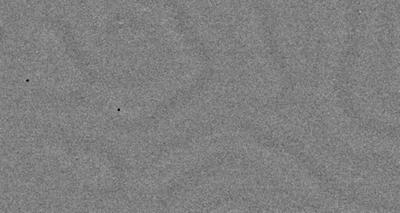
\includegraphics[width=0.13\textwidth]{prise_0100_resized.jpg}&
	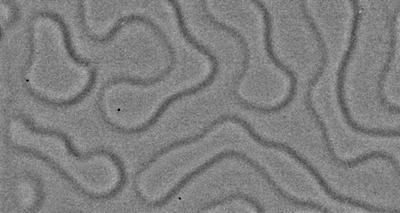
\includegraphics[width=0.13\textwidth]{prise_0130_resized.jpg}&
	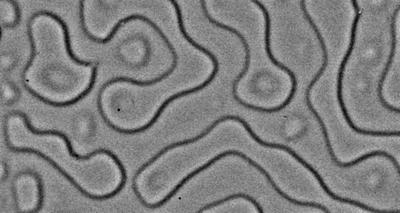
\includegraphics[width=0.13\textwidth]{prise_0160_resized.jpg}&
	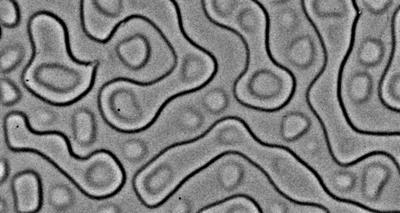
\includegraphics[width=0.13\textwidth]{prise_0190_resized.jpg}&
	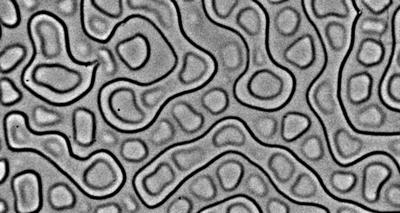
\includegraphics[width=0.13\textwidth]{prise_0250_resized.jpg}&
	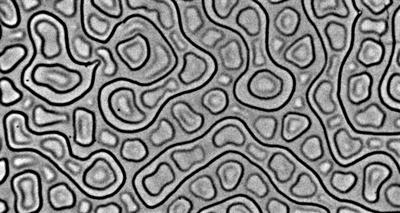
\includegraphics[width=0.13\textwidth]{prise_0360_resized.jpg}&
	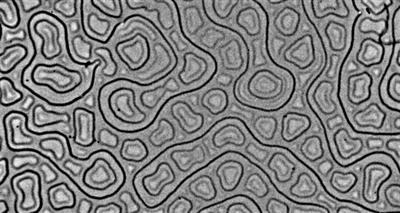
\includegraphics[width=0.13\textwidth]{prise_0799_resized.jpg}\\
	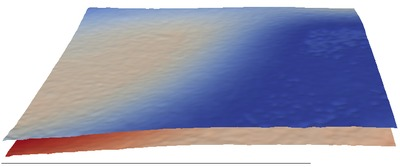
\includegraphics[width=0.13\textwidth]{cas3p2_fluo0p8_GDL4_2_t047_crop_resized.jpg}&
	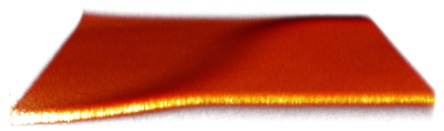
\includegraphics[width=0.13\textwidth]{cas3p2_fluo0p8_GDL4_2_t056_crop_resized.jpg}&
	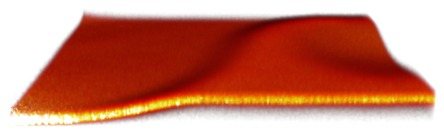
\includegraphics[width=0.13\textwidth]{cas3p2_fluo0p8_GDL4_2_t065_crop_resized.jpg}&
	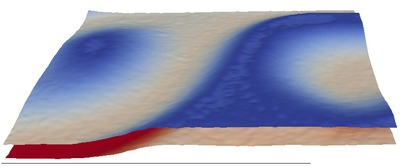
\includegraphics[width=0.13\textwidth]{cas3p2_fluo0p8_GDL4_2_t074_crop_resized.jpg}&
	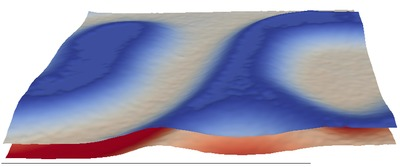
\includegraphics[width=0.13\textwidth]{cas3p2_fluo0p8_GDL4_2_t092_crop_resized.jpg}&
	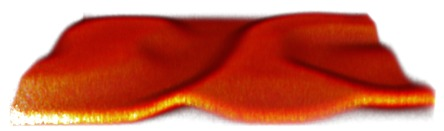
\includegraphics[width=0.13\textwidth]{cas3p2_fluo0p8_GDL4_2_t125_crop_resized.jpg}&
	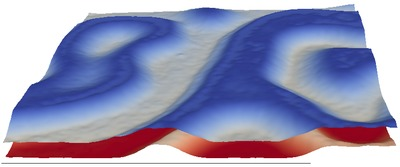
\includegraphics[width=0.13\textwidth]{cas3p2_fluo0p8_GDL4_2_t260_crop_resized.jpg}\\
	};
	\draw[ultra thick] ++(m-2-1.south west) -- ++(0.023\textwidth,0);
	\draw[ultra thick] ++(m-3-1.south west) -- ++(0.1\textwidth,0);
%	\begin{tabular*}{\textwidth}{@{\extracolsep{\fill}}p{2\TPHorizModule}llllll}
%	33 min\hfill \begin{tikzpicture}[inner sep=0]
%		\draw[ultra thick] (0,0) -- ++(0.355\TPHorizModule,0) node[pos=0.5, above=0, font=\small] {\SI{1}{\centi\metre}};
%	\end{tikzpicture}&
%	 38 min & 43 min & 48 min & 1h & 1h15 & 2h30\\
	
	\end{tikzpicture}
	\caption{Dynamics of pattern formation for $e\approx\SI{100}{\micro\metre}$. (top) By light transmission microscopy. (bottom) Reconstructed from fluorescent confocal microscopy. Scale bars are \SI{1}{\milli\metre}.}
	\label{fig:dynamics}
\end{figure*}

\end{document}